\documentclass{article}
\usepackage{anyfontsize}
\usepackage{tikz}
\begin{document}
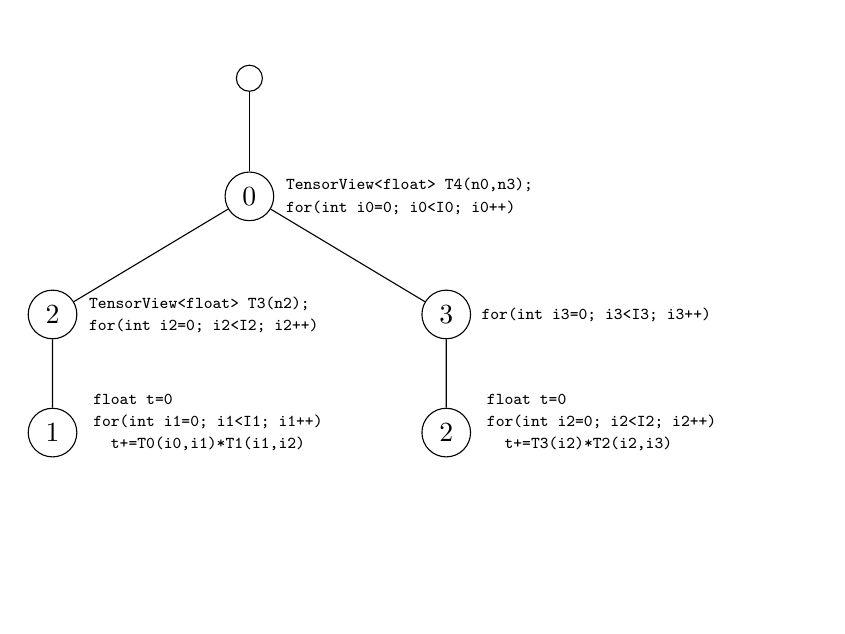
\begin{tikzpicture}[every node/.style={circle,draw=black},sibling distance=5cm]
\node{}
  child{
  node[label={[font=\fontsize{6pt}{8pt}\selectfont]right:\parbox{4cm}{\texttt{TensorView<float> T4(n0,n3);\\for(int i0=0; i0<I0; i0++)
}}}]{0}
    child{
    node[label={[font=\fontsize{6pt}{8pt}\selectfont]right:\parbox{4cm}{\texttt{TensorView<float> T3(n2);\\for(int i2=0; i2<I2; i2++)
}}}]{2}
      child{
      node[label={[font=\fontsize{6pt}{8pt}\selectfont]right:\parbox{4cm}{\texttt{float t=0\\ 
for(int i1=0; i1<I1; i1++)\\ 
\phantom{MM}t+=T0(i0,i1)*T1(i1,i2)\\}}}]{1}
      }
    }
    child{
    node[label={[font=\fontsize{6pt}{8pt}\selectfont]right:\parbox{4cm}{\texttt{for(int i3=0; i3<I3; i3++)
}}}]{3}
      child{
      node[label={[font=\fontsize{6pt}{8pt}\selectfont]right:\parbox{4cm}{\texttt{float t=0\\ 
for(int i2=0; i2<I2; i2++)\\ 
\phantom{MM}t+=T3(i2)*T2(i2,i3)\\}}}]{2}
      }
    }
  }
;
\end{tikzpicture}

 \end{document}
